% XCircuit output "basic_ADC.tex" for LaTeX input from basic_ADC.ps
\def\putbox#1#2#3{\makebox[0in][l]{\makebox[#1][l]{}\raisebox{\baselineskip}[0in][0in]{\raisebox{#2}[0in][0in]{#3}}}}
\def\rightbox#1{\makebox[0in][r]{#1}}
\def\centbox#1{\makebox[0in]{#1}}
\def\topbox#1{\raisebox{-\baselineskip}[0in][0in]{#1}}
\def\midbox#1{\raisebox{-0.5\baselineskip}[0in][0in]{#1}}
\begin{flushleft}
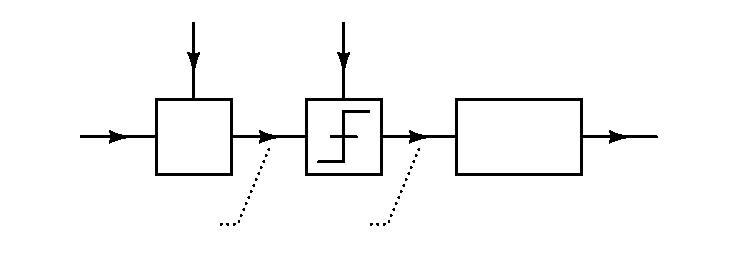
\epsfig{file=basic_ADC.ps}\\
% translate x=616 y=331 scale 0.38
\putbox{2.26in}{1.11in}{$\Delta$}%
\putbox{1.26in}{1.11in}{$T_s$}%
\putbox{4.35in}{0.65in}{$x(n)$}%
\putbox{0.06in}{0.65in}{$x_a(t)$}%
\putbox{0.85in}{0.07in}{$x_a(nT_s)$}%
\putbox{3.06in}{0.78in}{BINARY}%
\putbox{3.01in}{0.53in}{ENCODER}%
\putbox{1.06in}{0.65in}{S/H}%
\putbox{1.64in}{0.07in}{$\mathcal{Q}\bigl[x_a(nT_s)\bigr]$}%
\end{flushleft}
